\section{Characterizing Transnational Detours}
\label{datasets}
In this section, we describe our measurement methods, the challenges in
conducting them, and our findings concerning the transnational detours
of default Internet paths.

\begin{figure*}[t]
\centering
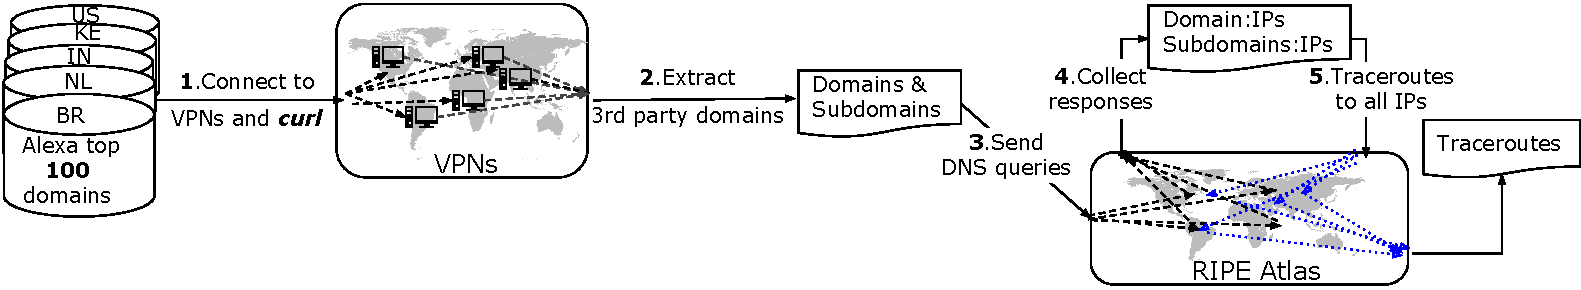
\includegraphics[width=.9\textwidth]{Current-Traffic_fig}
\caption{Measurement pipeline to study Internet paths from countries to
  popular domains.}
\label{fig:pipeline1}
\end{figure*}


\subsection{Measurement Pipeline}
\label{pipeline}

Figures \ref{fig:pipeline1} and \ref{fig:analysis_pipeline} summarize
our measurement process.  We analyze traceroute measurements to
discover which countries are on the path from a client in a particular
country to a popular domain.  
%JEN: repetitive
%Using traceroutes to measure
%transnational detours is new; prior work used BGP routing tables to
%\textit{infer} country-level paths~\cite{karlin2009nation}.  
Because we conduct active measurements, which are limited by our
resources, we study just five countries.  We report on measurements
conducted on January 31, 2016.

\subsubsection{Resource Limitations}
\label{resource_limits}

The iPlane~\cite{madhyastha2006iplane} and Center for Applied Internet
Data Analysis (CAIDA)~\cite{caida} projects maintain large
repositories of traceroute data, neither of which are suitable for our
study.  
%iPlane has historical data as far back as 2006.
Unfortunately, because iPlane uses PlanetLab~\cite{PlanetLab} nodes,
which mostly use the Global Research and Education Network (GREN), 
iPlane measurements are not be representative of typical Internet
users' traffic paths~\cite{banerjee2004interdomain}.  CAIDA runs
traceroutes from different vantage points around the world to
randomized destination IP addresses that cover all /24s; in contrast,
we focus on paths to popular websites from a particular country.

Instead, we run active measurements that
would represent paths of a typical Internet user. To do so, we run
DNS and traceroute measurements from RIPE Atlas probes, which are hosted
all around the world and in many different settings, including home
networks~\cite{ripe_atlas}.  RIPE Atlas probes can use the local DNS
resolver, which would give us the best estimate of the traceroute
destination.

Yet, conducting measurements from a RIPE Atlas probe costs a certain
amount of ``credits'', which restricts the number of measurements that we
could run.  RIPE Atlas also imposes rate limits on the number of
concurrent measurements and the number of credits that an individual
user can spend per day.  We address these challenges in two ways: (1)~we
reduce the number of necessary measurements we must run on RIPE Atlas
probes by conducting traceroute measurements to a single IP address in
each /24 (as opposed to all IP addresses returned by DNS) because all IP
addresses in a /24 belong to the same AS, and should therefore be
located in the same geographic area; (2)~we use a different method---VPN
connections---to obtain a vantage point within a foreign country, which
is still representative of an Internet user in that country.

\subsubsection{Path Asymmetry}
\label{path_sym}

The reverse path is just as important as (and often different from) the 
forward path.  
Previous work has shown that paths are not symmetric most of the
time---the forward path from point A to point B does not match the
reverse path from point B to point A~\cite{he2005routing}.  Most work on
path asymmetry has been done at the AS level, but not at the country
level.  Our measurements consider only the forward path (from client
to domain or relay), not the reverse path from the domain or
relay to the client.   

We measured path asymmetry at the country
granularity. If country-level paths are symmetric, then the results of
our measurements would be representative of the forward {\it and}
reverse paths. If the country-level paths are asymmetric, then our
measurement results only provide a lower bound on the number of countries
that could potentially conduct surveillance.  Using 100 RIPE Atlas
probes located around the world, and eight Amazon EC2 instances, we ran
traceroute measurements from every probe to every EC2 instance and from
every EC2 instance to every probe.  After mapping the IPs to countries,
we analyzed the paths for symmetry.  First, we compared the set of
countries on the forward path to the set of countries on the reverse
path; this yielded about 30\% symmetry.  What we wanted to know is
whether or not the reverse path has more countries on it than the
forward path.  Thus, we measured how many reverse paths were a subset of the
respective forward path; this was the case for 55\% of the paths.   
This level of asymmetry suggests that our results represent a lower
bound on the number of countries that transit traffic; our results are a
lower bound on how many unfavorable countries transit a client's
path. It also suggests that while providing lower bounds on
transnational detours is feasible, designing systems to completely
prevent these detours on both forward and reverse paths may be particularly
challenging, if not impossible. 

\subsubsection{Traceroute Origin and Destination Selection}

Each country hosts a different number of RIPE Atlas probes, ranging
from about 75 probes to many hundreds.  Because of the resource
restrictions, we could not use all probes in each of the countries.  We
selected the set of probes that had unique ASes in the country to get
the widest representation of origination (starting) points.

For destinations, we used the Alexa Top 100 domains in each of the
respective countries, as well as the third-party domains that are
requested as part of an original web request.  To obtain these 3rd party
domains we {\tt curl} (\ie, HTTP fetch) each of the domains, but we must
do so from within the country of interest.  There is no current
functionality to {\tt curl} from RIPE Atlas probes, so we establish a
VPN connection within each of these countries to {\tt curl} each domain
and extract the third-party domains; we {\tt curl} from the client's
location in case web sites are customizing content based on the region
of the client. 

\begin{figure}[t]
\centering
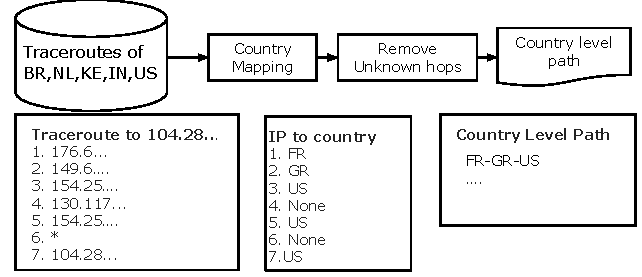
\includegraphics[width=.5\textwidth]{Analysis-Pipeline1}
\caption{Mapping country-level paths from traceroutes.}
\label{fig:analysis_pipeline}
\end{figure}


\subsubsection{Country Mapping}
\label{c_map}

Accurate IP geolocation is challenging. We use MaxMind's
geolocation service to map IP addresses to their respective
countries~\cite{maxmind}, which is known to contain inaccuracies.
Fortunately, our study does not require high-precision geolocation; we
are more interested in providing accurate lower bounds on detours at a
much coarser granularity.  Fortunately, previous work has found that
geolocation at a country-level granularity is more accurate than at
finer granularity~\cite{huffaker2011geocompare}.  In light of these
concerns, we post-processed our IP to country mapping
by removing all IP addresses that resulted in a `None' response when
querying MaxMind, which causes our results to provide a conservative
estimate of the number of countries that paths traverse. It is important
to note that removing `None' responses will \textit{always} produce a
conservative estimate, and therefore we are \textit{always}
underestimating the amount of potential surveillance.  
Figure \ref{fig:analysis_pipeline} shows an example of this
post-processing. 

\subsection{Results}


%%%% ADD THIS TO datasets.tex
\newcolumntype{d}[1]{D{.}{.}{#1}}
\newcommand{\headrow}[1]{\multicolumn{1}{c}{\adjustbox{angle=45,lap=\width-0.5em}{#1}}}
\newcolumntype{P}[1]{>{\raggedright\arraybackslash}p{#1}}
\newcommand{\ra}[1]{\renewcommand{\arraystretch}{#1}}
\begin{table}[t]
\centering
\ra{1}
\resizebox{\columnwidth}{!}{%
\begin{tabular}{@{}ld{3.2}d{3.2}d{3.2}d{3.2}d{3.2}@{}}
%\multicolumn{1}{l}{}    & \headrow{Host} & \headrow{Transit} & \headrow{Host} & \headrow{Transit} &\headrow{Host} &\headrow{Transit} &\headrow{Host}   &\headrow{Transit} &\headrow{Host}  &\headrow{Transit} \\
\textit{Terminating in Country} 
   & \headrow{Brazil}  & \headrow{Netherlands}   & \headrow{India} & \headrow{Kenya} & \headrow{United States}\\
\toprule
Brazil             &.169    &\multicolumn{1}{r}{-}     &\multicolumn{1}{r}{-}    &\multicolumn{1}{r}{-}  &\multicolumn{1}{r}{-} \\ \midrule
Canada             &.001    &.007     &.015      &.006       &\multicolumn{1}{r}{-}  \\
United States      &\cellcolor[HTML]{F7BE81}.774    &\cellcolor[HTML]{F7BE81}.454      &\cellcolor[HTML]{F7BE81}.629      &\cellcolor[HTML]{F7BE81}.443        &\cellcolor[HTML]{F7BE81}.969    \\ \midrule
France             &.001    &.022      &.009      &.023       &.001 \\
Germany            &.002    &.013      &.014      &.028       &.001  \\
Great Britain      &\multicolumn{1}{r}{-}  &.019     &.021     &.032       &.002 \\
Ireland            &.016    &.064      &.027       &.108       &.001   \\
Netherlands        &.013    &\cellcolor[HTML]{F7BE81}.392      &\cellcolor[HTML]{F7BE81}.101      &\cellcolor[HTML]{F7BE81}.200      &.024  \\
Spain              &.001    &\multicolumn{1}{r}{-}     &\multicolumn{1}{r}{-}    &\multicolumn{1}{r}{-}     &\multicolumn{1}{r}{-}    \\ \midrule
Kenya              &\multicolumn{1}{r}{-}        &\multicolumn{1}{r}{-}    &\multicolumn{1}{r}{-}    &.022        &\multicolumn{1}{r}{-}  \\
Mauritius          &\multicolumn{1}{r}{-}      &\multicolumn{1}{r}{-}    &\multicolumn{1}{r}{-}   &.004       &\multicolumn{1}{r}{-}  \\
South Africa       &\multicolumn{1}{r}{-}       &\multicolumn{1}{r}{-}     &\multicolumn{1}{r}{-}  &.021       &\multicolumn{1}{r}{-}  \\ \midrule
United Arab Emirates &\multicolumn{1}{r}{-}     &\multicolumn{1}{r}{-}     &\multicolumn{1}{r}{-}   &.011        &\multicolumn{1}{r}{-}  \\
India              &\multicolumn{1}{r}{-}      &\multicolumn{1}{r}{-}     &.053    &.002        &\multicolumn{1}{r}{-}  \\
Singapore          &\multicolumn{1}{r}{-}       &.002     &\cellcolor[HTML]{F7BE81}.103      &.027       &\multicolumn{1}{r}{-} \\\hline
\end{tabular}
}
\caption{Fraction of paths that terminate in each country by default.}
\label{tab:host}
\end{table}

\begin{table}[t]
\centering
\ra{1}
\resizebox{\columnwidth}{!}{%
\begin{tabular}{@{}ld{3.2}d{3.2}d{3.2}d{3.2}d{3.2}@{}}
%\multicolumn{1}{l}{}    & \headrow{Host} & \headrow{Transit} & \headrow{Host} & \headrow{Transit} &\headrow{Host} &\headrow{Transit} &\headrow{Host}   &\headrow{Transit} &\headrow{Host}  &\headrow{Transit} \\

\textit{Transiting Country}    & \headrow{Brazil}  & \headrow{Netherlands}   & \headrow{India} & \headrow{Kenya} & \headrow{United States}\\ \toprule
Brazil              &1.00       &\multicolumn{1}{r}{-}   &\multicolumn{1}{r}{-}     &\multicolumn{1}{r}{-}     &\multicolumn{1}{r}{-} \\ \midrule
Canada                &.013       &.007     &.016       &.008      &.081 \\
United States        &\cellcolor[HTML]{F7BE81}.844        &\cellcolor[HTML]{F7BE81}.583     &\cellcolor[HTML]{F7BE81}.715      &\cellcolor[HTML]{F7BE81}.616       &\cellcolor[HTML]{F7BE81}1.00 \\ \midrule
France                 &.059     &.102      &.104       &.221      &.104 \\
Germany                 &.005       &.050    &.032      &.048      &.008 \\
Great Britain                &.024       &\cellcolor[HTML]{F7BE81}.140     &\cellcolor[HTML]{F7BE81}.204      &\cellcolor[HTML]{F7BE81}.500      &.006 \\
Ireland                &.028       &.106      &.031     &.133      &.006 \\
Netherlands                 &.019        &1.00      &.121      &\cellcolor[HTML]{F7BE81}.253      &.031 \\
Spain                  &.176       &.004     &\multicolumn{1}{r}{-}     &\multicolumn{1}{r}{-}      &\multicolumn{1}{r}{-} \\ \midrule
Kenya                 &\multicolumn{1}{r}{-}       &\multicolumn{1}{r}{-}    &\multicolumn{1}{r}{-}      &1.00      &\multicolumn{1}{r}{-} \\
Mauritius                  &\multicolumn{1}{r}{-}       &\multicolumn{1}{r}{-}     &\multicolumn{1}{r}{-}      &\cellcolor[HTML]{F7BE81}.322       &\multicolumn{1}{r}{-} \\
South Africa                 &\multicolumn{1}{r}{-}        &\multicolumn{1}{r}{-}    &\multicolumn{1}{r}{-}     &\cellcolor[HTML]{F7BE81}.334       &\multicolumn{1}{r}{-} \\ \midrule
United Arab Emirates                  &\multicolumn{1}{r}{-}        &\multicolumn{1}{r}{-}    &\multicolumn{1}{r}{-}     &.152       &\multicolumn{1}{r}{-} \\
India               &\multicolumn{1}{r}{-}    &\multicolumn{1}{r}{-}    &1.00     &.058     &\multicolumn{1}{r}{-} \\
Singapore                 &\multicolumn{1}{r}{-}        &.002     &\cellcolor[HTML]{F7BE81}.270       &.040       &.003 \\ \midrule
\end{tabular}
}
\caption{Fraction of paths that each country transits by default.}
\label{tab:transit}
\end{table}


Table \ref{tab:host} shows the five countries we studied along the top
of the table, and the countries that host their content along in each
row.  For example, the U.S. is the endpoint of 77\% of the
paths that originate in Brazil.  A ``-'' represents the case where no
paths ended in that country.  For example, no Brazilian paths terminated in
South Africa. Table \ref{tab:transit} shows the fraction of paths that
transit (or end in) certain countries, with a row for each country that is transited.

\begin{finding}[Hosting Diversity]
About half of the top domains in each of the five countries studied are hosted in a single country.  The other half are located in two or more different countries.
\end{finding}
\noindent
First we analyze hosting diversity; this shows us how many unique
countries host a domain.  The more countries that a domain is hosted
in creates a greater chance that the content is replicated in a
favorable country, and could potentially allow a client to circumvent
an unfavorable country.  We queried DNS from 26 vantage points around
the world, in geographically diverse locations.  Then we
mapped the IP addresses in the DNS responses to countries to determine
how many unique countries host a domain.  Figure~\ref{fig:host_diversity} shows the fraction of domains that are hosted in different numbers of countries; we can see two common hosting cases: 1) CDNs and 2) a single hosting country.  This shows that many domains are hosted in a single unique country, which leads us to our next analysis---where are these domains hosted, and which countries are traversed on the way to reach these locations.

%\begin{figure}[t]
%\centering
%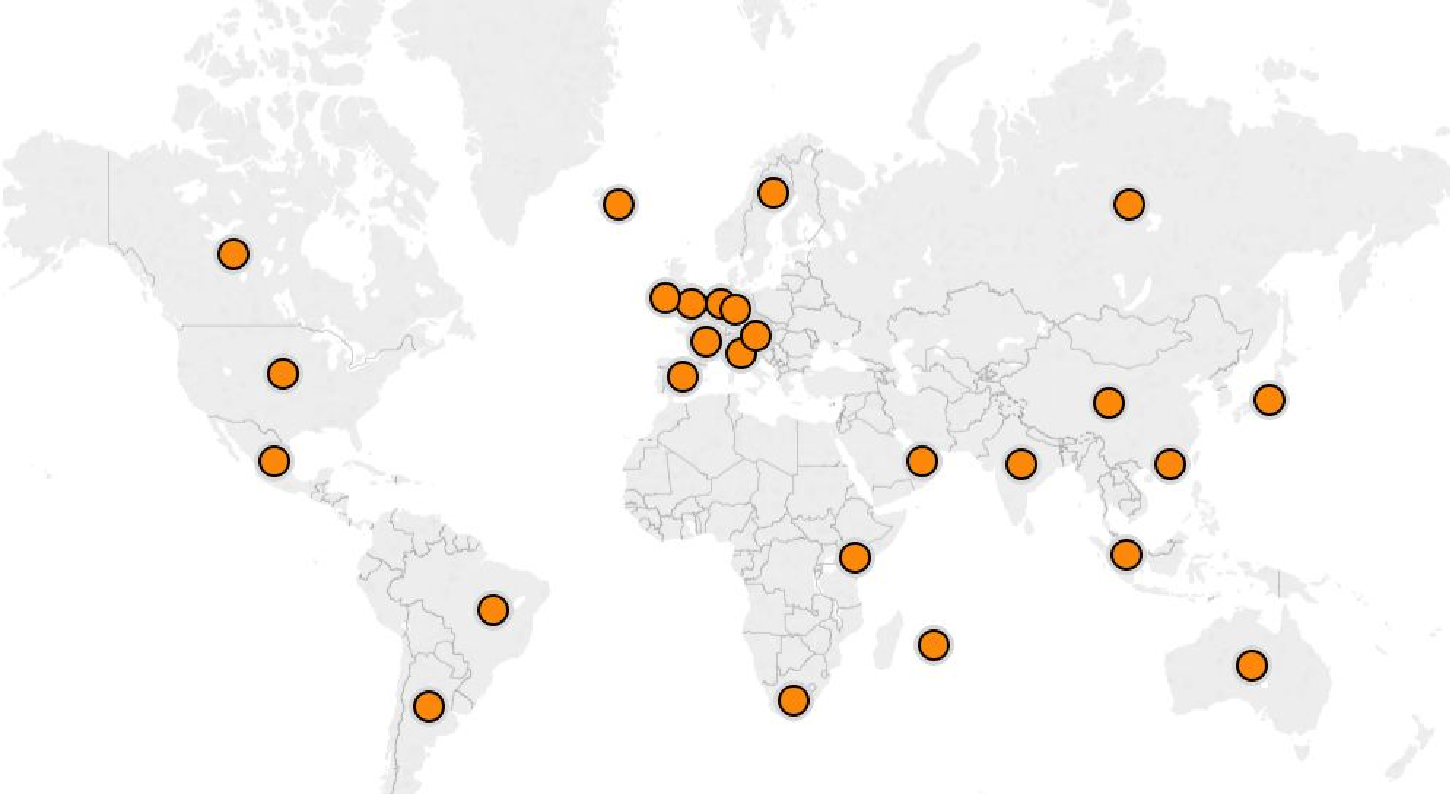
\includegraphics[width=0.8\columnwidth]{World-DNS}
%\caption{Vantage points in measuring hosting diversity.}
%\label{fig:world}
%\end{figure}

\begin{figure}[t]
\centering
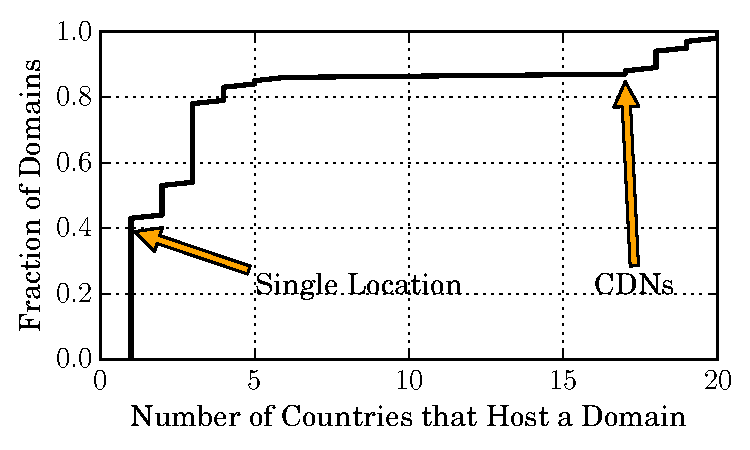
\includegraphics[width=.8\columnwidth]{domain_hist_US1}
\caption{The number of Alexa Top 100 US Domains hosted in different countries.}
\label{fig:host_diversity}
\end{figure}


\begin{figure*}[t!]
\begin{minipage}{\linewidth}
\begin{subfigure}[b]{.32\linewidth}
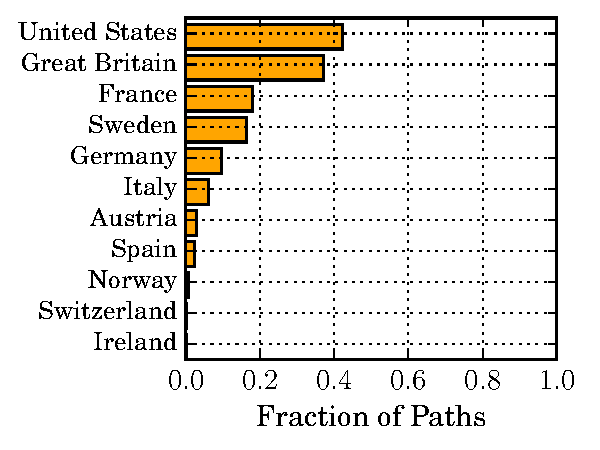
\includegraphics[width=\linewidth]{nl_trombone_new11}
\caption{The Netherlands.\label{fig:trombone_netherlands}}
\end{subfigure}
\begin{subfigure}[b]{.32\linewidth}
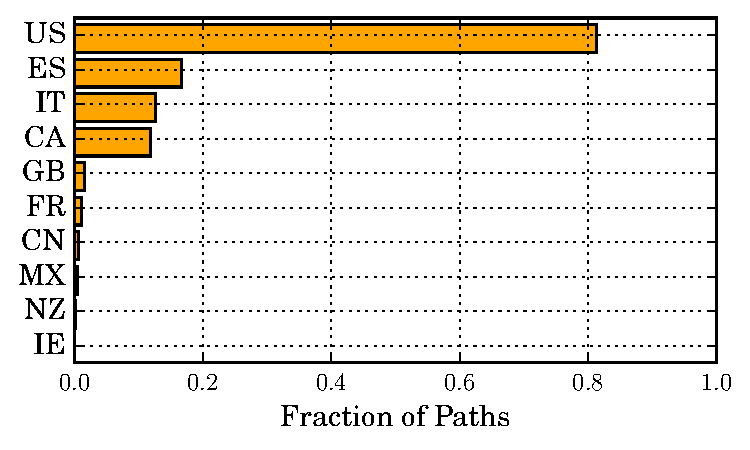
\includegraphics[width=\linewidth]{br_trombone_new11}
\caption{Brazil.\label{fig:trombone_brazil}}
\end{subfigure}
\begin{subfigure}[b]{.32\linewidth}
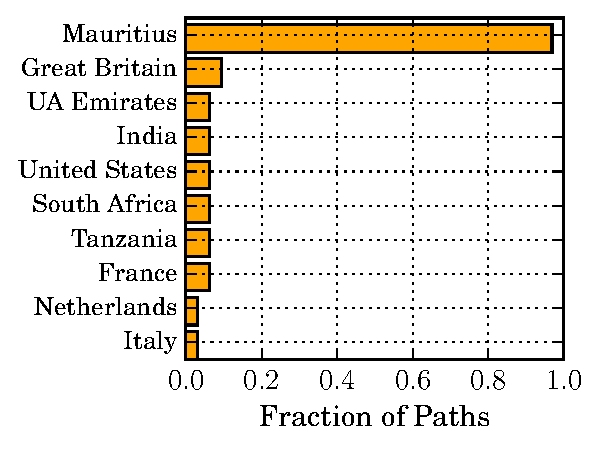
\includegraphics[width=\linewidth]{ke_trombone_new11}
\caption{Kenya.\label{fig:trombone_kenya}}
\end{subfigure}
\end{minipage}
\caption{The countries that tromboning paths from the Netherlands, Brazil, and Kenya transit.}
\label{fig:trombone}
\end{figure*}



\begin{finding}[Domain Hosting]
The most common destination among all five countries studied is the U.S.: 77\%, 45\%, 63\%, 44\%, and 97\% of paths originating in Brazil, Netherlands, India, Kenya and the U.S., respectively, are currently reaching content located in the U.S.
\end{finding}
\noindent
Table~\ref{tab:host} shows the fraction of paths that are hosted in
various countries.  Despite the extent of country-level hosting
diversity, the majority of paths from all five countries terminate in a
single country: the United States, a known surveillance state.   Our results also show the Netherlands is a
common hosting location for paths originating in the Netherlands, India,
and Kenya.

%For Indian traffic, in addition to the 63\% hosted in the United States and the 10\% hosted in the Netherlands, another 10\% is hosted in Singapore.  Hosting in these countries can best be explained by the number of underwater cables with landing points in both India and Singapore~\cite{cablemap}.  More specifically, there is a cable that directly connects Chennai, India and Changi North, Singapore, and is owned by Tata Communications, which is one of the top global Internet providers (in terms of transited IP space)~\cite{bakers}.  

%For Kenyan traffic, the United States hosts 44\% of the content, but Ireland hosts 10\%; Ireland is a popular hosting location for U.S. companies due to its relaxed enforcement of privacy in the private sector \annie{I got this information from Joel Reidenberg - how do I cite that?  I'll also look to see if I can find any publications that discuss this}.  

\begin{finding}[Domestic Traffic]
All of the countries studied (except for the United States) host content for a small percentage of the paths that originate in their own country; they also host a small percentage of their respective country-code top-level domains.
\end{finding}
\noindent
Only 17\% of paths that originate in Brazil also end there.  Only 5\%
and 2\% of Indian and Kenyan paths, respectively, end in the originating
country.  
For Kenya, 24 out of the Top 100 Domains are .ke domains, but only 5
of the 24 are hosted within Kenya.  29 out of 40 .nl domains are hosted in the Netherlands; 4 of 13 .in domains are hosted in India; 18 of 39 .br domains are hosted in Brazil.  Interestingly, all .gov domains were hosted in their respective country. 

\begin{finding}[Transit Traffic]
Surveillance states (specifically the U.S. and Great Britain) are on the largest portion of paths in comparison to any other (foreign) country.
\end{finding}
\noindent
84\% of Brazilian paths traverse the United States, despite Brazil's
strong efforts to avoid United States surveillance.  Although India and
Kenya are geographically distant, 72\% and 62\% of their paths also transit
the United States.

Great Britain and the Netherlands are on the path for a significant
percentage of paths originating in India and Kenya: 50\% and 20\% of
paths that originate in Kenya and India, respectively, transit Great
Britain.   Many paths likely traverse Great Britain and the Netherlands due to
the presence of large Internet Exchange Points (\ie, LINX, AMS-IX).
Mauritius, South Africa, and the United Arab Emirates transit 32\%,
33\%, and 15\% of paths from Kenya.  There are direct underwater cables
from Kenya to Mauritius, and from Mauritius to South
Africa~\cite{cablemap}.  Additionally, there is a cable from Mombasa,
Kenya to Fujairah, United Arab Emirates, which likely explains the large
fraction of paths that include these countries. 



\begin{finding}[Tromboning Traffic]
Brazilian and Netherlands paths often trombone to the United States, despite the prevalence of IXPs in both countries.
\end{finding}
\noindent
Figures \ref{fig:trombone}
shows the fraction of paths that trombone to
different countries for the Netherlands, Brazil, and Kenya. 24\% of
all paths originating in the Netherlands (62\% of domestic paths)
trombone to a foreign country before returning to the
Netherlands. Despite Brazil's strong efforts in building IXPs to keep
local traffic local, 
their paths still trombone to the U.S.  This is due to IXPs being seen
as a threat by competing commercial providers; providers are sometimes
concerned that ``interconnection'' will result in making business
cheaper for competitors and stealing of customers~\cite{ixp_policy}.
It is likely that Brazilian providers see one another as competitors and therefore as a threat at IXPs, which causes them to peer with international providers instead of other local providers.  Additionally, we see Brazilian paths trombone to Spain and Italy. We have observed that MaxMind sometimes mislabels IP addresses to be in Spain when they are actually located in Portugal.  This mislabelling does not affect our analysis of detours through surveillance states, as we do not highlight either Spain or Portugal as a surveillance state.  We see Italy often in tromboning paths because Telecom Italia Sparkle is one of the top global Internet providers~\cite{bakers}.

Tromboning Kenyan paths most commonly traverse Mauritius, which is expected considering the submarine cables between Kenya and Mauritius.  Submarine cables also explain South Africa, Tanzania, and the United Arab Emirates on tromboning paths.  
  %Traffic that should be kept local is susceptible to surveillance because it transits two well-known surveillance states.  

\begin{finding}[United States as an Outlier]
The United States hosts 97\% of the content that is accessed from within the country, and only five foreign countries---France, Germany, Ireland, Great Britain, and the Netherlands---host content for the other 3\% of paths.
\end{finding}
\noindent
Many of the results find that Brazilian,
Netherlands, Indian, and Kenyan paths often transit surveillance states,
most notably the U.S.  The results from studying paths that
originate in the U.S. are drastically different from those of
the other four countries.  The other four countries host very small
amounts of content accessed from their own country, whereas the U.S.
hosts 97\% of the content that is accessed from within the
country.  Only 13 unique countries are ever on a path from the U.S.
to a domain in the top 100 (or third party domain), whereas 30,
30, 25, and 38 unique countries are seen on the paths originating in
Brazil, Netherlands, India, and Kenya, respectively.   

%There are only 6 foreign countries---France, Germany, Ireland, Great Britain, and the Netherlands----that host content for traffic originating in the United States, and the fraction of content hosted in these countries is less than 4\% combined.

\subsection{Limitations}

This section discusses the various limitations of our measurement methods
and how they may affect our results.

\paragraph{Traceroute accuracy and completeness.}
Our study is limited by the accuracy and completeness of traceroute.
Anomalies can occur in traceroute-based
measurements~\cite{augustin2006avoiding}, but most traceroute anomalies
do not cause an overestimation in surveillance states.  The
incompleteness of traceroutes, where a router does not respond, causes
our results to underestimate the number of surveillance states, and
therefore also provides a lower bound on surveillance. 

\paragraph{IP geolocation vs.\ country mapping.}
There are fundamental challenges in deducing a geographic location
from an IP address, 
%JEN: remove the details about methods?
despite using different methods such as DNS names of the target,
network delay measurements, and host-to-location mapping in
conjunction with BGP prefix
information~\cite{padmanabhan2001investigation}.  While there are
inaccuracies and incompleteness in MaxMind's
data~\cite{huffaker2011geocompare}, the focus of this work is on
measuring and avoiding surveillance.  We use Maxmind to map IP to
country,
% (as described in Section~\ref{c_map}),
which provides a lower
bound on the amount of surveillance.

\paragraph{IPv4 vs.\ IPv6 connectivity.}
We collect and analyze only IPv4 paths.  IPv6 paths likely
differ from IPv4 paths as not all routers that support IPv4 also support
IPv6.  Future work includes studying IPv6 paths.  

